%%%%%%%%%%%%%%%%%%%%%%%%%%%%%%%%%%%%%%%%%%%%%%%%%%%%%%%%%%%%%%%%%%%%%%%%%%%%%%%%%%%%%%%%%%%%%%%%%%%%

\chapter{Details on The Molecular Outflow in \ngc253 at a Resolution of Two Parsecs}
\chaptermark{Details on the molecular outflow}
\label{appendix: outflow}

%%%%%%%%%%%%%%%%%%%%%%%%%%%%%%%%%%%%%%%%%%%%%%%%%%%%%%%%%%%%%%%%%%%%%%%%%%%%%%%%%%%%%%%%%%%%%%%%%%%%


\section{Kinematic model of the central molecular gas}
\label{appendix: outflow: model}

We derive a model for the velocity of the disk component from the \co10 observations using the kinematic fitting tool \texttt{diskfit} \citep{2007ApJ...664..204S,2010MNRAS.404.1733S,2015arXiv150907120S}. As mentioned in Section~\ref{outflow: subsection: ppV separation}, these models benefit from large area which is why we base them on the \co10 observations. A $20\sigma$ threshold ensures that the model is fitted to the bright disk excluding any fainter outflows.

In \texttt{diskfit}, we fit using the velocity field fitter. The names of the set options in \texttt{diskfit} are given in paratheses in the following. The model is fitted to all pixels within an ellipse of $75\arcsec$ major axis length (\texttt{regrad}), $\mathrm{PA} = 53^\circ$ (\texttt{regpa}) and ellipticity $\epsilon = 0.66$ (\texttt{regeps}). Outside this range, we use a sampling factor of 2 pixels (\texttt{istepout}). During the fit, the center is held fixed while we fit for disk position angle and ellipticity with initial guesses of $\mathrm{PA} = 53^\circ$ and $\epsilon = 0.66$ based on by eye inspection (line 9 and 10 of the parameter file). We allow the model to fit for non-axisymmetric flows with $\mathrm{PA} = 78^\circ$ initial guess and order $m=2$ (line 12) which means \texttt{diskfit} will fit for rotation plus a bisymmetric model with $m=2$ perturbations to the potential (bar). As the \co10 data cover the kinematic center we set the inner interpolation toggle to true which assumes the velocity raises linearly within the innermost fitted ring. We do not fit for radial flows (radial flows toggle) because it allows to many degrees of freedom and produces bad models as is warned about in the \texttt{diskfit} manual. We further fit for the systemic velocity and exclude warps from the model. A model with these parameters is fitted in rings at radii $12.5\arcsec$, $25\arcsec$, $37.5\arcsec$, $50\arcsec$, $62.5\arcsec$, $75\arcsec$, $87.5\arcsec$, $100\arcsec$, $125\arcsec$, $150\arcsec$, $175\arcsec$, $200\arcsec$, $225\arcsec$, $250\arcsec$, $275\arcsec$ and $300\arcsec$.

The residuals show a slight mismatch in velocity of $\sim 20-30$\,\kms along the direction of the bar. This is likely due to the bar being underestimated because the \co10 image covers only the inner half of the total extent of the bar. The mismatch gets larger when fitting a model to the smaller images of \co21 and (3--2) which confirms that it is caused by lack of observed area. We fit this mismatch in the velocity field with an additional 2D Gaussian component and add it to the velocity field of the diskfit model to obtain a better model. Note that this additional component is not physically motivated or meaningful but purely aims to counteract the effect of limited observation area.

Figure~\ref{outflow: figure: model} shows the velocity field of the model in comparison to the input \co10 velocity field. The model typically fits the observed velocity field better than $\pm 25$\,\kms; larger deviations occur mostly over small areas of order one beam size. The model thus successfully reproduces the large scale velocity field.


\begin{figure*}
	\centering
	\includegraphics[scale=0.18]{images/chapters/papers/outflow/outflow_figA1a.pdf}
	\includegraphics[scale=0.18]{images/chapters/papers/outflow/outflow_figA1b.pdf}\\
	\includegraphics[scale=0.18]{images/chapters/papers/outflow/outflow_figA1c.pdf}
	\includegraphics[scale=0.18]{images/chapters/papers/outflow/outflow_figA1d.pdf}
	\caption[Observed and modeled velocity field]{Input data and model represented as velocity fields. \emph{top left}: \co10 velocity field to which the model is fitted, known foreground emission is removed; \emph{top right}: model velocity field; \emph{bottom left}: \co10 velocity overlaid with model contours; \emph{bottom right}: residual velocity. The velocity fields use the same colorscale from 100\,\kms to 400\,\kms with contours in steps of 50\,\kms within that range. The residual velocity uses the same colorscale relative to the systemic velocity of 250\,\kms with contours from -50\,\kms to +50\,\kms in steps of 25\,\kms.}
	\label{outflow: figure: model}
\end{figure*}


%%%%%%%%%%%%%%%%%%%%%%%%%%%%%%%%%%%%%%%%%%%%%%%%%%%%%%%%%%%%%%%%%%%%%%%%%%%%%%%%%%%%%%%%%%%%%%%%%%%%
%%%%%%%%%%%%%%%%%%%%%%%%%%%%%%%%%%%%%%%%%%%%%%%%%%%%%%%%%%%%%%%%%%%%%%%%%%%%%%%%%%%%%%%%%%%%%%%%%%%%

\section{Velocity width of the disk mask}
\label{appendix: outflow: disk velocity range}

The definition of the disk mask is crucial for this analysis as it determines if a molecular cloud is considered kinematically consistent with the disk or if it is potentially outflowing. The position of the disk mask in ppV space is set by the disk model but the width (velocity range $\Delta v$) of the mask is a free parameter. From Figure~\ref{outflow: figure: all pV diagrams} it is obvious that $\Delta v$ depends on the distance from the major axis which is most simply accounted for by a parametrisation of form $\Delta v = a \exp \left( -\left( \frac{x}{b} \right)^2 \right) +c$. Finding the best fit values for $a, b$ and $c$ is difficult to do mathematically as the fit would need to be on the disk component that we want to determine from the mask first. We therefore select values that visually fit the pV diagrams as best as possible. They are given in equation~\ref{equation: delta v}.

Figure~\ref{outflow: figure: disk mask width} shows five alternative masks that vary only in width by 10\% from the best fit mask. It is apparent that even slight changes of 10\% deteriorate the fit between mask and disk emission. More narrow masks obviously do not cover all disk emission whereas the wider masks include spike features that are kinematically inconsistent with disk rotation.

\begin{figure}
    \centering
    \includegraphics[width=\textwidth]{images/chapters/papers/outflow/outflow_figB1.pdf}
    \caption[Effect of varying pV slice width]{Position-velocity diagrams for the central slice along the major axis (offset 0.0\arcsec) overlaid with five different choices for the velocity width of the disk mask. Greyscale and overlays are identical to Figure~\ref{outflow: figure: sample slice} and \ref{outflow: figure: all pV diagrams}. The central panel shows the visually best fitting mask as defined by equation~\ref{equation: delta v}. The other panels use masks of 80\%, 90\%, 110\% and 120\% of the best fit width. Even 10\% change in mask width lead to noticeable mismatch in the high-resolution \co32 data.}
    \label{outflow: figure: disk mask width}
\end{figure}{}

The effect of a $^{+10}_{-10}$\% ($^{+0.04}_{-0.04}$\,dex) variation in mask velocity width results in a $^{+0.01}_{-0.01}$\,dex change in integrated disk luminosity for \co10, \co21 and \co32. The non-disk components is less bright than the disk and thus shows a higher relative variation when changing the mask width: luminosities vary by $^{-0.07}_{+0.08}$\,dex ($^{-0.06}_{+0.07}$\,dex, $^{-0.11}_{+0.12}$\,dex) for \co10 (\co21, \co32). Note the inverse scaling between disk and non-disk due to shifting the balance between the two components for a constant total luminosity. To first order, the same percentage changes apply to the further quantities mass, outflow rate, energy and momentum.


%%%%%%%%%%%%%%%%%%%%%%%%%%%%%%%%%%%%%%%%%%%%%%%%%%%%%%%%%%%%%%%%%%%%%%%%%%%%%%%%%%%%%%%%%%%%%%%%%%%%
%%%%%%%%%%%%%%%%%%%%%%%%%%%%%%%%%%%%%%%%%%%%%%%%%%%%%%%%%%%%%%%%%%%%%%%%%%%%%%%%%%%%%%%%%%%%%%%%%%%%

\section{Disk/non-disk separation: Position-velocity diagrams}
\label{appendix: outflow: all pVs}

Figure~\ref{outflow: figure: all pV diagrams} shows all pV diagrams for the slices defined in Figure~\ref{outflow: figure: slice positions}. For the discussion of these diagrams, see Section~\ref{outflow: section: disk separation}.

\vspace{0.5cm}

\begin{figure}[ht!]
	\centering
	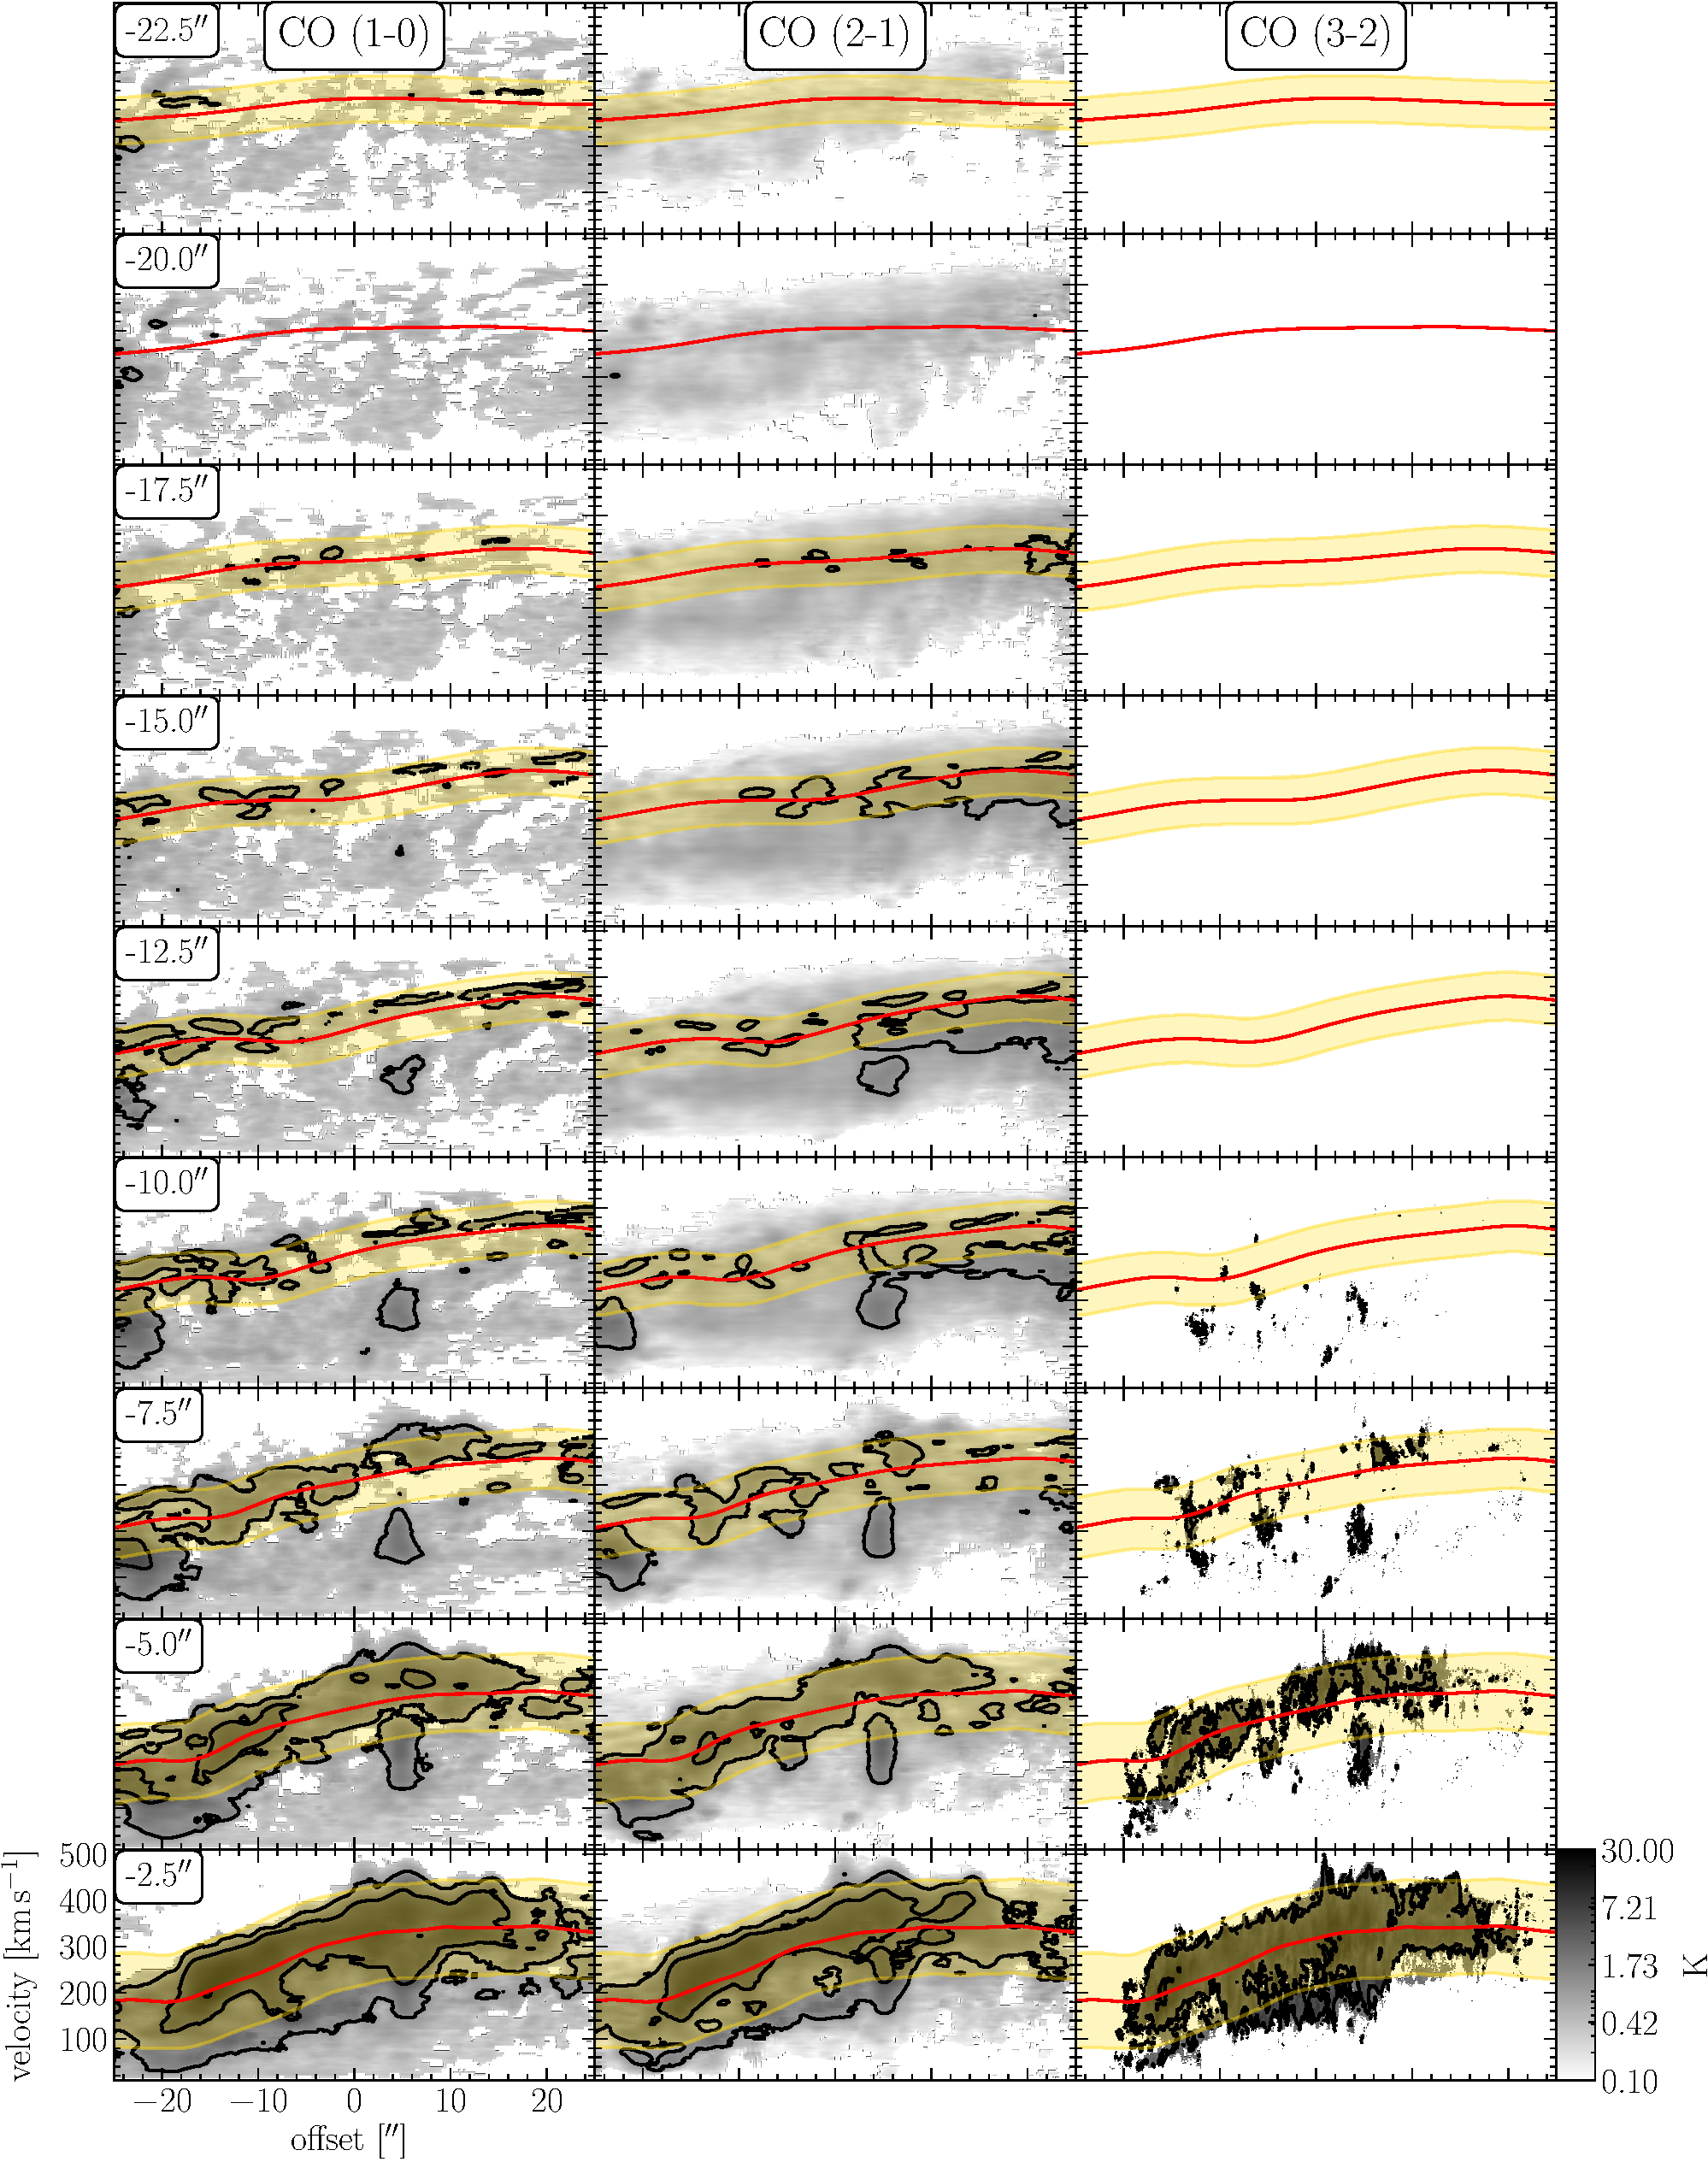
\includegraphics[width=\textwidth]{images/chapters/papers/outflow/outflow_figC1a.pdf}
	\caption[Complete list of pV slices]{Position-velocity diagrams for all slices defined in Section~\ref{outflow: section: disk separation} and Figure~\ref{outflow: figure: slice positions} for \co10, \co21 and \co32 in the left to right column. A description of the overlays is given in Figure~\ref{outflow: figure: sample slice}.}
	\label{outflow: figure: all pV diagrams}
\end{figure}

\begin{figure}
	\ContinuedFloat
	\centering
	\includegraphics[width=\textwidth]{images/chapters/papers/outflow/outflow_figC1b.pdf}
	\caption[]{continued}
\end{figure}


%%%%%%%%%%%%%%%%%%%%%%%%%%%%%%%%%%%%%%%%%%%%%%%%%%%%%%%%%%%%%%%%%%%%%%%%%%%%%%%%%%%%%%%%%%%%%%%%%%%%
%%%%%%%%%%%%%%%%%%%%%%%%%%%%%%%%%%%%%%%%%%%%%%%%%%%%%%%%%%%%%%%%%%%%%%%%%%%%%%%%%%%%%%%%%%%%%%%%%%%%